% Format teze zasnovan je na paketu memoir
% http://tug.ctan.org/macros/latex/contrib/memoir/memman.pdf ili
% http://texdoc.net/texmf-dist/doc/latex/memoir/memman.pdf
% 
% Prilikom zadavanja klase memoir, navedenim opcijama se podešava 
% veličina slova (12pt) i jednostrano štampanje (oneside).
% Ove parametre možete menjati samo ako pravite nezvanične verzije
% mastera za privatnu upotrebu (na primer, u b5 varijanti ima smisla 
% smanjiti 
\documentclass[12pt,oneside]{memoir} 

% Paket koji definiše sve specifičnosti master rada Matematičkog fakulteta
\usepackage[latinica]{matfmaster} 
\usepackage{elm-highlighting}
\usepackage{lmodern}
\usepackage{listings,xcolor}

\usepackage[T1]{fontenc}
\usepackage{xcolor}
\usepackage[scaled=0.9]{DejaVuSansMono}

\lstdefinestyle{DOS}
{
    backgroundcolor=\color{black},
    basicstyle=\scriptsize\color{white}\ttfamily
}
\definecolor{commentgreen}{RGB}{2,112,10}
\definecolor{eminence}{RGB}{108,48,130}
\definecolor{weborange}{RGB}{255,165,0}
\definecolor{frenchplum}{RGB}{129,20,83}

\lstdefinelanguage{elixir}{
    morekeywords={case,catch,def,do,else,false,%
        use,alias,receive,timeout,defmacro,defp,%
        for,if,import,defmodule,defprotocol,%
        nil,defmacrop,defoverridable,defimpl,%
        super,fn,raise,true,try,end,with,field,type%
        unless, |>, <-, \}, \{, \%, ->},
 %   otherkeywords={->},
    sensitive=true,
    morecomment=[l]{\#},
    morecomment=[n]{/*}{*/},
    morecomment=[s][\color{purple}]{:}{\ },
    morestring=[s][\color{orange}]"",
    commentstyle=\color{commentgreen},
    keywordstyle=\color{eminence},
    stringstyle=\color{red},
	basicstyle=\ttfamily,
	breaklines,
	showstringspaces=false,
	frame=tb
}


%

%

%
% Opcija [biblatex]:
%   ako želite da koristite reference na više jezika i umesto paketa
%   bibtex da koristite BibLaTeX/Biber, dodajte opciju "biblatex" tj.
%   prethodni paket uključite pomoću: \usepackage[biblatex]{matfmaster}
%
% Opcija [b5paper]:
%   ako želite da napravite verziju teze u manjem (b5) formatu, navedite
%   opciju "b5paper", tj. prethodni paket uključite pomoću: 
%   \usepackage[b5paper]{matfmaster}. Tada ima smisla razmisliti o promeni
%   veličine slova (izmenom opcije 12pt na 11pt u \documentclass{memoir}).
%
% Naravno, opcije je moguće kombinovati.
% Npr. \usepackage[b5paper,biblatex]{matfmaster}


% Datoteka sa literaturom u BibTex tj. BibLaTeX/Biber formatu
\bib{matfmaster-primer}

% Ime kandidata na srpskom jeziku (u odabranom pismu)
\autor{Ana Petrović}
% Naslov teze na srpskom jeziku (u odabranom pismu)
\naslov{Testiranje softvera u funkcionalnim programskim jezicima Elm i Elixir}
% Godina u kojoj je teza predana komisiji
\godina{2023}
% Ime i afilijacija mentora (u odabranom pismu)
\mentor{dr Milena \textsc{Vujošević Janičić}, redovan profesor\\ Univerzitet u Beogradu, Matematički fakultet}
% Ime i afilijacija prvog člana komisije (u odabranom pismu)
\komisijaA{dr Filip \textsc{Marić}, vanredni profesor\\ Univerzitet u Beogradu, Matematički fakultet}
% Ime i afilijacija drugog člana komisije (u odabranom pismu)
\komisijaB{dr Ivan \textsc{Čukić}, docent\\ Univerzitet u Beogradu, Matematički fakultet}
% Ime i afilijacija trećeg člana komisije (opciono)
% \komisijaC{}
% Ime i afilijacija četvrtog člana komisije (opciono)
% \komisijaD{}
% Datum odbrane (odkomentarisati narednu liniju i upisati datum odbrane ako je poznat)
% \datumodbrane{}

% Apstrakt na srpskom jeziku (u odabranom pismu)
\apstr{%
Apstrakt
}

% Ključne reči na srpskom jeziku (u odabranom pismu)
\kljucnereci{funkcionalno programiranje, testiranje, verifikacija softvera, programski jezik Elixir, programski jezik Elm}

\begin{document}
% ==============================================================================
% Uvodni deo teze
\frontmatter
% ==============================================================================
% Naslovna strana
\naslovna
% Strana sa podacima o mentoru i članovima komisije
\komisija
% Strana sa posvetom (u odabranom pismu)
%\posveta{Mami, tati i dedi}
% Strana sa podacima o disertaciji na srpskom jeziku
\apstrakt
% Sadržaj teze
\tableofcontents*

% ==============================================================================
% Glavni deo teze
\mainmatter
% ==============================================================================

% ------------------------------------------------------------------------------
\chapter{Uvod}
% ------------------------------------------------------------------------------
\par
Ovde ide uvod .. ... ..... 
\par uvod uvod

\par sta se nalazi u kom poglavlju...


% ------------------------------------------------------------------------------
\chapter{Funkcionalna paradigma}
\label{chp:uvodnideo}

\par Funkcionalno programiranje je specifičan pristup programiranju, tj. programska paradigma, koja se zasniva na pojmu matematičke funkcije. Programi se kreiraju pomoću izraza i funkcija, bez izmena stanja i podataka \cite{func}. Iz tog razloga, jednostavniji su za razumevanje i otporniji na greške u odnosu na imperativne programe. Programski stil je deklarativnog tipa i umesto naredbi koriste se izrazi, tako da se izvršavanje programa svodi na evaluaciju izraza. Vrednost izraza je nezavisna od konteksta u kojem se izraz nalazi, što se naziva \emph{transparentnost referenci} i predstavlja osnovnu osobinu \emph{čistih} funkcionalnih jezika (eng. \textit{pure functional programming language}). Transparentnost referenci kao osnovnu posledicu ima nepostojanje propratnih efekata. Sa druge strane, \emph{nečisti} funkcionalni jezici (eng. \textit{impure functional programming language}) dozvoljavaju propratne efekte, koji mogu izazvati suptilne greške i biti teži za razumevanje. Međutim, praktičniji su za specifične vrste zadataka, kao što je programiranje korisničkog interfejsa ili rad sa bazom podataka. 
%\par Funkcionalni jezici zasnovani su na \textit{lambda računu} (eng. \textit{$\lambda$-calculus}), čija je osnovna svrha da d\a'a  definiciju izračunljivosti. Pored toga što se smatra prvim %funkcionalnim jezikom, lambda račun se naziva i najmanjim programskim jezikom na svetu. Sve što se može izračunati lambda računom smatra se izračunljivim. Ekspresivnost % funkcionalnih jezika ekvivalentna je ekspresivnosti Tjuringove mašine \cite{turing}. 
% TODO ako se ovo iybacuje, izbaciti literaturu


\section{Karakteristike funkcionalnih jezika}
U nastavku su objašnjene neke od najvažnijih osobina jezika funkcionalne paradigme. 

\subsection{Funkcije kao građani prvog reda}
U funkcionalnim programima, funkcije se smatraju građanima prvog reda (eng. \emph{first class citizen}). To znači da u okviru jezika ne postoje restrikcije po pitanju njihovog kreiranja i korišćenja. Građani prvog reda su entiteti u okviru programskog jezika koji mogu biti:
\begin{itemize}
\item deo nekog izraza
\item dodeljeni nekoj promenljivoj
\item prosleđeni kao argument funkcije
\item povratne vrednosti funkcije
\end{itemize}
Mogućnost prosleđivanja funkcija kao argumenata drugih funkcija je ključna za funkcionalnu paradigmu. 

\subsection{Čista funkcija}
\par  Čista funkcija (eng. \textit{pure function}) ima dve osnovne karakteristike: 
\begin{itemize}
\item Transparentnost referenci 
\item Imutabilnost 
\end{itemize}
\par  Koncept transparetnosti referenci se odnosi na to da je vrednost izraza jedinstveno određena. Izraz se može zameniti svojom vrednošću na bilo kom mestu u programu, bez promene u ponašanju programa. Definicija se može proširiti i na funkcije: funkcija poseduje transparentnost referenci ako pri pozivu sa istim vrednostima argumenata uvek proizvodi isti rezultat. Ponašanje takve funkcije je određeno njenim ulaznim vrednostima.
\par Imutabilnost podrazumeva odsustvo propratnih efekata, tj. da čista funkcija ne vrši nikakve izmene nad argumentima, kao ni nad promenljivima. Jedini rezultat čiste funkcije jeste vrednost koju ona vrati. Kao posledica ovoga, funkcionalni programi su laki za debagovanje. Čiste funkcije takođe olakšavaju paralelizaciju i konkurentnost aplikacija. Na osnovu ovako napisanih programa, kompilator lako može da paralelizuje naredbe, sačeka da evaluira rezultate kada budu potrebni, i na kraju da zapamti rezultat, s obzirom na to da se on neće promeniti sve dok ulaz ostaje isti. K$\hat{o}$d \ref{lst:pure} prikazuje primer jedne čiste funkcije u programskom jeziku Elixir. 

\begin{lstlisting}[language=elixir, caption={Primer čiste funkcije},captionpos=b, label={lst:pure}]
defmodule Math do 
  def fibonacci(0) do 0 end
  def fibonacci(1) do 1 end
  def fibonacci(n) do fibonacci(n-1) + fibonacci(n-2) end
end

IO.puts Math.fibonacci(9)
\end{lstlisting}

\subsection{Funkcije višeg reda}
Funkcija višeg reda je funkcija koja kao argument uzima jednu ili više funkcija i/ili ima funkciju kao svoju povratnu vrednost. U funkcionalnom programiranju se intenzivno koriste ovakve funkcije, a po svojoj važnosti se posebno izdvajaju \textit{map}, \textit{filter} i \textit{reduce (fold)}.  Funkcija \textit{map} kao argumente prima funkciju i listu, i zatim primeni datu funkciju na svaki element liste i kao povratnu vrednost proizvodi novu listu. Upotrebom funkcije \textit{filter} mogu se eliminisati neželjeni elementi neke liste --- na osnovu prosleđene funkcije predikata i date liste, \textit{filter} vraća listu sa elementima koji ispunjavaju dati kriterijum. \textit{Fold} prihvata tri argumenta: funkciju spajanja, početnu vrednost i listu. Iznova primenjuje funkciju spajanja na početnu vrednost i datu listu, sve dok se rezultat ne redukuje na jednu vrednost. 
\par Prednost korišćenja ovih funkcija je u sažetom i čistom kodu. Takođe, pogodne su i za paralelizaciju. Primer koda \ref{lst:high} pokazuje upotrebu funkcija višeg reda u programskom jeziku Elm.


\begin{lstlisting}[language=elm, caption={Funkcije višeg reda},captionpos=b, label={lst:high}]
[1, 2, 3] |> List.map (\number -> number * 2) -- [2, 4, 6]
[1, 2, 3, 4, 5] |> List.filter (\number -> number <= 3) -- [1, 2, 3]
[1, 2, 3, 4, 5] |> List.foldl (\item total -> total + item) 0 -- 15
\end{lstlisting}

\subsection{Odsustvo promenljivih i rekurzija}
\par Čisti funkcionalni jezici nemaju stanje koje bi se menjalo tokom izvršavanja programa, pa zbog toga ne podržavaju koncept promenljivih. Sa druge strane, nečisti funkcionalni jezici podržavaju i karakteristike drugih programskih paradigmi, te je u okviru njih dozvoljena upotreba promenljivih. Iako su fleksibilniji po tom pitanju, nečisti funkcionalni jezici promovišu imutabilnost kao dobru praksu. 
\par Kod funkcionalno napisanih programa može se primetiti odsustvo petlji. Funkcije se definišu rekurzivno --- pozivaju same sebe i time postižu ponavljanje izvršavanja. U mnogim slučajevima, umesto rekurzije se koriste funkcije višeg reda.

\section{Testiranje u razvoju softvera}
\label{sec:piramid}

\par Testiranje koda je jedan od najvažnijih aspekata u procesu razvoja softvera. Cilj testiranja je pronalaženje grešaka, proverom da li su ispunjeni svi funkcionalni i nefunkcionalni zahtevi \cite{test}.  Softver koji ne radi onako kako je predviđeno može dovesti do različitih problema, kao što su gubitak novca i vremena, ili u najgorim slučajevima --- povrede ili smrti. Testiranjem se osigurava kvalitet softvera i smanjuje rizik od neželjenog ponašanja. Glavna uloga testiranja jeste verifikacija softvera --- provera da li sistem zadovoljava specifikaciju, ali uključuje i validaciju --- proveru da li sistem ispunjava sve potrebe korisnika.  

%\par Razvoj vođen testovima (eng. \emph{Test-Driven Development , TDD}) je praksa u razvoju softvera koja nalaže da se prvo napišu testovi. Ti testovi na početku ne prolaze, s obzirom na to da k$\hat{o}$d još uvek nije implementiran, a zatim se iznova pokreću tokom pisanja samog koda, sve dok ne prođu. Ova tehnika kontinualnog testiranja tokom razvoja se često preporučuje jer se lako i veoma rano uoče greške i time sprečavaju u kasnijim fazama razvoja. Ipak, u ovom radu neće biti primenjen TDD pristup. Kako je tema testiranje, fokus nije na pisanju koda aplikacije, već testova za već napisan projekat. Aplikacija koja će biti testirana služi samo kao primer na kome će biti prikazani značajni koncepti testiranja funkcionalnih programa. Kratak opis testiranog projekta biće preciznije objašnjen u poglavlju \ref{chp:msnr}. 

\subsection{Organizacija testova}
\par Model piramide testiranja (prikazan na slici \ref{fig:piramida}) je koncept koji pomaže u razmišljanju o tome kako testirati softver \cite{cohn}. Uloga piramide je da vizuelno predstavi logičku organizaciju standarda u testiranju. Sastoji se od tri sloja: bazu piramide predstavljaju jedinični testovi (eng. \emph{unit test}). Njih bi trebalo da bude najviše --- kako su najmanji, samim tim su i najbrži, a izvršavaju se u potpunoj izolaciji. Na sledećem nivou, u sredini piramide, nalaze se integracioni testovi. Integracija podrazumeva način na koji različite komponente sistema rade zajedno. Nisu potrebne interakcije sa korisničkim interfejsom, s obzirom na to da ovi testovi pozivaju k$\hat{o}$d preko interfejsa. Vrh piramide čine sistemski testovi. Oni se ne fokusiraju na individualne komponente, već testiraju čitav sistem kao celinu i time utvrđuju da on radi očekivano i ispunjava sve funkcionalne i nefunkcionalne zahteve. Takvi testovi su prilično skupi, pa je potrebno doneti odluku koliko, i koje od njih se isplati sprovesti.
\par Jedna vrsta sistemskih testova su takozvani E2E testovi\footnote{E2E je skraćenica za testove sa kraja na kraj (eng. \emph{end-to-end})}, koji simuliraju korisničko iskustvo kako bi osigurali da sistem funkcioniše kako treba, od korisničkog interfejsa, pa sve do serverske strane i baze podataka. Testovi korisničkog interfejsa (eng. \emph{User Interface tests, UI tests}) se staraju o tome da se korisnički interfejs ponaša na očekivan način. Obično su automatski i simuliraju interakcije pravih korisnika sa aplikacijom, kao što su pritiskanje dugmića, unos teksta i slično. S obzirom na to da oni proveraju da sistem, zajedno sa svojim korisničkim interfejsom, radi kako treba --- mogu se u određenom kontekstu smatrati sistemskim testovima, ali su ipak specifičniji i mogu se sprovoditi i nezavisno od celokupnog sistema. 
\par U opštem slučaju, testiranje projekta koji se sastoji od više slojeva podrazumeva kombinaciju jediničnih, integracionih i sistemskih testova kako bi se osigurala ukupna funcionalnost, pouzdanost i perfomanse sistema.

\begin{figure}[!ht]
  \centering
  \label{fig:piramida}
  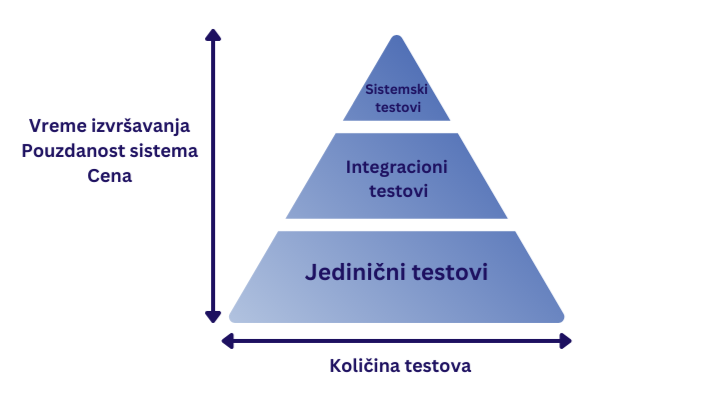
\includegraphics[width=0.8\textwidth]{piramidanova.png}
  \caption{Model piramide testiranja}
\end{figure}

\subsubsection{Testovi jedinica koda}
\par Jedinica je mala logička celina koda: može biti funkcija, klasa, metod klase, modul i slično. Jedinični test proverava samo da li se data jedinica ponaša prema svojoj specifikaciji. Ovi testovi se mogu pisati u potpunoj izolaciji, i ne zavise ni od jedne druge komponente, servisa, ni korisničkog interfejsa. Dakle, izdvajaju se najmanji testabilni delovi aplikacije i proverava se da li rade ono za šta su namenjeni. Ovi testovi su najjednostavniji za pisanje jer se bave malim delom aplikacije, te je k$\hat{o}$d koji se testira najčešće vrlo jednostavan. 
\par Cilj jediničnih testova jeste da spreče greške koje mogu nastati izmenama koda, kao i da omoguće da se lako utvrdi lokacija dela koda koji izaziva grešku. Pri dizajniranju ovih testova, potrebno je proveriti da k$\hat{o}$d radi tačno ono za šta je namenjen, a da se to uradi pisanjem najmanje moguće dodatne količine koda.

\subsubsection{Anatomija jediničnih testova}
\par Kako bi k$\hat{o}$d jediničnog testa bio čitljiv i jednostavan za razumevanje, obrazac četvorofaznog testa (eng. \emph{four-phase test}) predlaže strukturu testa koja podrazumeva ne više od četiri faze \cite{4phase}. Svaki test jedinice koda se može podeliti na četiri jasno odvojive celine:  
\begin{enumerate}
\item Priprema (eng. \emph{setup}) --- sređivanje podataka koji će se prosleđivati pred samu proveru (uglavnom nije neophodno u testiranju čisto funkcionalnih programa).
\item Delovanje (eng. \emph{exercise}) --- pozivanje koda koji se testira, ključni deo svakog testa.
\item Verifikacija (eng. \emph{verify}) --- testovi proveravaju ponašanje koda (često se spaja sa prethodnom fazom). 
\item Rušenje (eng. \emph{teardown}) --- vraćanje podataka na prvobitno stanje, npr. ako se u prvoj fazi koriste neka deljena stanja, kao što je baza podataka. Ovaj korak se često izvršava implicitno. 
\end{enumerate}

\par Konkretan primer ovako organizovanog testa u programskom jeziku Elm dat je u primeru \ref{lst:4ph}. Definisan je jednostavan test, koji proverava da li funkcija koja sabira dva broja daje ispravan rezultat. U fazi pripreme brojevima i njihovoj očekivanoj sumi se dodeljuju vrednosti . U fazi delovanja poziva se funkcija \emph{sum}, a pozivanjem funkcije \emph{expect} proverava se da li je rezultat jednak očekivanom u fazi verifikacije. Faza rušenja u ovom slučaju ne treba da uradi ništa.

\begin{lstlisting}[language=elm, caption={Četiri faze jediničnog testa koji proverava ispravnost
funkcije sabiranja dva broja},captionpos=b, label={lst:4ph}]
import Test exposing (..)

sumTest : Test
sumTest =
    describe "sum" [
      test "should add two numbers correctly" <| \() -> 
        let
        --Setup
           x = 2
           y = 3
           expected = 5
        in
        -- Exercise (sum)
        -- Verify (expect)
           expect (sum x y) |> toEqual expected
    ]

   -- Teardown
   teardown : Int -> ()
   teardown _ =
    ()
\end{lstlisting}

\subsubsection{Integracioni testovi}
\label{sec:integration}
\par Jedan od ključnih koraka u razvoju softvera jeste pisanje integracionih testova. Oni utvrđuju da li različite komponente sistema rade zajedno na predviđen način. Pojedinačni moduli i komponente se kombinuju i testiraju kao jedna celina. Cilj integracionog testiranje jeste identifikacija i rešavanje problema koji mogu nastati nakon što se komponente softverskog sistema integrišu i krenu da međusobno komuniciraju. Svaka od njih pojedinačno možda radi kako treba, ali nakon što se to utvrdi jediničnim testovima, potrebno je proveriti da li će njihova interakcija izazvati neželjeno ponašanje. 
\par U zavisnosti od potreba konkretnog sistema, postoje različiti pristupi integracionom testiranju. Ako su komponente viših nivoa kritične za funkcionalnost sistema, ili od njih zavisi mnogo drugih komponenti, ima smisla prvo testirati njih, pa kasnije postepeno preći na komponente nižih nivoa. Ovakav pristup se naziva testiranje odozgo nadole (eng. \emph{top-down integration testing}). U suprotnom, ako su komponente nižih slojeva arhitekture kritičnije za celokupan sistem, predlaže se testiranje odozdo nagore (eng. \emph{bottom-up integration testing}). Hibridno integraciono testiranje (eng. \emph{hybrid integration testing}) podrazumeva kombinaciju prethodna dva --- započinje sa testovima komponenti najvišeg sloja, zatim se prelazi na testiranje najnižeg sloja, sve dok se postepeno ne stigne do središnjih. Kada je sistem relativno jednostavan i ne postoji veliki broj komponenti, može se primeniti pristup po principu ''velikog praska'' (eng. \emph{big-bang integration testing}), koji podrazumeva testiranje svih komponenti odjednom, kao jedne celine. 
\par Ako se komponente nalaze u okviru istog sistema, gde postoji kontrola i neko očekivano ponašanje --- integracioni testovi su prilično jednostavni. Međutim, kada su u pitanju spoljašnje komponente i testiranje interakcije sistema sa njima, pisanje integracionih testova postaje malo komplikovanije. Mnoge aplikacije koriste baze podataka, druge servise ili API-je, sa kojima se testovi moraju uskladiti. U testovima se mogu koristiti pravi podaci, ili se umesto njih ubaciti takozvani dubleri (eng. \textit{test doubles}).
\par Integraciono testiranje je neophodno da bi se obezbedio kvalitetan i pouzdan softver, i zahvaljujući njemu rano se uočavaju različiti problemi do kojih može doći i time značajno redukuje vreme i cena celokupnog razvoja. 


\subsubsection{Sistemski testovi}
\label{sec:system}
\par Nakon završenog jediničnog i integracionog testiranja, neophodno je sprovesti sistemske testove. Ova vrsta testiranja se vrši nad kompletno integrisanim sistemom, i podrazumeva proveru da li celokupni sistem ispunjava zahteve, odnosno da li je spreman za isporuku krajnjim korisnicima. Sistemski testovi se sprovode u okruženju koje je konfigurisano tako da bude što sličnije onom kakvo će biti u produkciji. Praksa je da ih pišu testeri koji nisu učestvovali u razvoju, kako bi se izbegla pristrasnost. Pored funkcionalnih i nefunkcionalnih specifikacija koje se tiču ponašanja sistema, testiraju i očekivanja korisnika. Mogu biti manuelni ili automatski. 
\par Sistemsko testiranje se smatra testiranjem crne kutije (eng. \emph{black-box testing}). Ponašanje sistema se evaluira iz ugla korisnika, što znači da ne zahteva nikakvo znanje o unutrašnjem dizajnu i strukturi koda. Ono što je neophodno jeste da očekivanja i zahtevi budu precizni i jasni, kao i da se razume upotreba aplikacije u realnom vremenu. 
\par Postoji mnogo vrsta sistemskog testiranja, i potrebno je doneti odluku koje od njih će biti sprovedene, u zavisnosti od zahteva, tipa aplikacije i raspoloživih resursa.  Neke od vrsta sistemskog testiranja koje se odnose na nefunkcionalne osobine softvera su: 
\begin{itemize}
\item Testiranje oporavka (eng. \emph{recovery testing}) --- nakon što se izazove pad sistema, proverava se da li se on vraća u prvobitno stanje na ispravan način.
\item Testiranje perfomansi (eng. \emph{perfomance testing}) --- proverava se skalabilnost, pouzdanost, i vreme odgovora sistema.
\item Testiranje sigurnosti (eng. \emph{security testing}) --- proverava se da li je sistem adekvatno zaštićen od upada ili gubitka podataka. 
\item Regresiono testiranje (eng. \emph{regression testing}) --- proverava se da li su se pojavile neke naknadne greške pri dodavanju novih funkcionalnosti. 
\item Testiranje kompatibilnosti (eng. \emph{compatibility testing}) --- proverava se da li sistem radi ispravno u različitim okruženjima, npr. kada se koristi na drugom hardveru ili operativnom sistemu.
\end{itemize}
\par Pisanjem sistemskih testova obezbeđuje se kvalitet i pouzdanost softvera, umanjuje rizik od neispravnosti i povećava zadovoljostvo korisnika sistema. Temeljnim testiranjem sistema mogu se otkriti i ispraviti novi problemi pre samog puštanja u rad, koje nije bilo moguće primetiti u ranijim fazama testiranja. 

\section{Testiranje funkcionalnih programa}

\par Najvažnija stvar kod testiranja u funkcionalnoj paradigmi jeste pisanje čistih funkcija i njihovo testiranje u izolaciji, kako bi se obezbedila ispravnost i robustnost. Takođe je važno da se ne testira samo uspešan scenario, već i granični slučajevi, kao i slučajevi greške.

\subsection{Testiranje čistih funkcija}

\par Najjednostavniji k$\hat{o}$d za testiranje jeste čista funkcija. Pri testiranju čiste funkcije, s obzirom da ne postoje propratni efekti, test može da se fokusira samo na dve stvari: ulazne podatke i na sam izlaz funkcije. 
\par Kada je u pitanju čista funkcija, jedina priprema koja je potrebna jesu podaci koji će se proslediti kao parametri. Drugi korak jeste poziv funkcije, sa prosleđenim argumentima. Faza verfikacije podrazumeva samo provere nad rezultatom. Testovi su veoma jednostavni jer ne moraju da brinu o propratnim efektima i njihovim neželjenim posledicama.
\par Aplikacije se u većini slučajeva neće sastojati od isključivo čistih funkcija, i u vezi sa tim postoje dve strategije \cite{testingelixir}. Prva je izdvojiti logiku u čiste funkcije, a druga dizajnirati funkcije tako da koriste neku od metoda ubrizgavanja zavisnosti (eng. \textit{dependency injection}) \footnote{Ubrizgavanje zavisnosti je obrazac u kom objekat ili funkcija prihvata druge objekte ili funkcije od kojih zavisi. Jedan od oblika inverzije kontrole, za cilj ima da razdvoji konstrukciju i upotrebu objekata i time smanjuje spregnutost programa.}, što omogućava izolaciju koda.

\subsubsection{Refaktorisanje ka čistim funkcijama} 
Ako je neki deo koda komplikovan za testiranje, najlakši način da se pojednostavi jeste refaktorisati ga u čistu funkciju, ukoliko je to moguće. Deo koda koji zavisi od nekog drugog dela iz spoljašnjosti će u većini slučajeva pozivati tu spoljašnju zavisnost i onda manipulisati rezultatom pre nego što vrati svoj rezultat. Što više takve manipulacije ima, to je taj deo koda bolji kandidat za premeštanje logike unutar čiste funkcije. Na slici \ref{fig:dep} su date vizuelne reprezentacije kako ovaj proces izgleda pre i posle izmeštanja koda u čistu funkciju. 
Na početku, funkcija može biti komplikovana za testiranje. Svaki test, za svaki mogući način ponašanja bi nekako morao da garantuje da druga funkcija (ona od koje zavisi prva) vraća neki očekivani odgovor. Ideja je da se deo logike (na slici označen sa ``manipulacija podataka ``) izvuče van --- u novu, čistu funkciju. Tako postaje zasebna komponenta, koja se može odvojeno lako testirati. Kada je taj deo logike dobro istestiran, može se smatrati sigurnim da se ponovo pozove u originalnoj funkciji. Zna se da će taj čisti k$\hat{o}$d uvek vraćati isti rezultat, i može se značajno redukovati broj testova neophodnih za testiranje originalne funkcije. U primeru koda... TODO primer

\begin{figure}[!ht]
  \centering
  \label{fig:dep}
  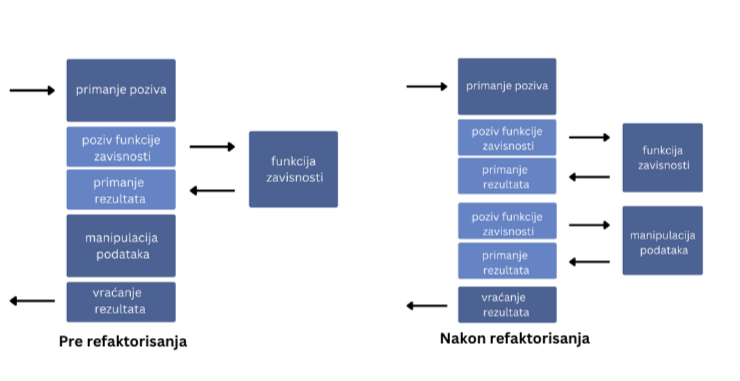
\includegraphics[width=0.9\textwidth]{dep.png}
  \caption{Izmeštanje koda u čistu funkciju}
\end{figure}

\par  U nekim slučajevima, nije lako odrediti šta se može izdvojiti u zasebnu funkciju. Tada postoji druga opcija za kreiranje kontrolisanog okruženja: napraviti zamenu za funkciju zavisnosti, i time izolovati k$\hat{o}$d. 

\subsection{Izolovanje koda} 
\par Ubrizgavanjem zavisnosti i kreiranjem dublera moguće je eliminisati spoljašnje promenljive, i time kontrolisati situaciju u kojoj k${o}$d koji se testira mora da se nađe. Tako se omogućava očekivanje nekog konkretnog rezultata. 
\par Zavisnost je bilo koji k$\hat{o}$d na koji se originalni k$\hat{o}$d oslanja. Korišćenjem DI (skraćenica za Dependency Injection) u testovima se kreiraju zamene zavisnosti koje se ponašaju na predvidljiv način, pa testovi mogu da se fokusiraju na logiku unutar koda koji se testira. U jediničnim testovima, najčešće se ubrizgava zavisnost tako što se prosledi kao parametar. Taj parametar može biti funkcija ili modul. Ubrizgavanje zavisnosti kroz API\footnote{skraćenica za aplikacioni veb interfejs (eng. \textit{web applicatoin
programming interface} )} obezbeđuje čist k$\hat{o}$d i jednostavne i kontrolisane jedinične testove. Sa druge strane, integracioni testovi zahtevaju drugačije metode ubrizgavanja zavisnosti. TODO nastavak...

% ------------------------------------------------------------------------------

\chapter{Portal MSNR}
\label{chp:msnr}

\par K$\hat{o}$d aplikacije pod nazivom \emph{Portal MSNR} koja će biti testirana javno je dostupan na \emph{GitHub-u} \cite{msnr-portal}. Portal MSNR je veb aplikacija namenjena praćenju i upravljanju aktivnostima kursa \emph{Metodologija stručnog i naučnog rada} \cite{rad}. Studenti na ovom kursu treba da steknu različite veštine koje se tiču pravilnog pisanja i recenziranja naučnih radova, pisanja CV-a, držanja prezentacija, i komunikacije u radu na timskim projektima. 

\section{Funkcionalnosti i osnovni entiteti portala}
\label{sec:entiteti}
\par Različite aktivnosti na kursu \emph{Metodologija stručnog i naučnog rada} implementirane su kao funkcionalnosti aplikacije. Korisnik portala može imati jednu od dve uloge: \emph{student} ili \emph{profesor}. Student na početku mora da podnese zahtev za registraciju, koju nakon toga odobrava profesor, i zatim student ima mogućnost da se prijavi na portal. Jedna od obaveza studenata na kursu jeste pisanje seminarskog rada --- profesor vrši odabir tema za tekuću godinu, a studenti treba da prijave svoju grupu za izradu seminarskog rada. Student ima i opciju da se prijavi za recenziranje radova drugih studenata, ukoliko to želi. Drugi zadatak koji se očekuje od studenata jeste pisanje CV-a. U okviru portala, student može priložiti tri različite vrste dokumenata --- prvu verziju seminarskog rada, recenzije, i svoju prvu verziju CV-a. Profesor, pored toga što vrši pregled zahteva za registraciju i odabir tema, ima mogućnost dodavanja svih aktivnosti tokom godine, i na kraju --- njihovo ocenjivanje.

\subsection{Entiteti}
\par Osnovni entiteti aplikacije predstavljeni su tabelama u bazi podataka i relacijama između njih.  Polazni entiteti su \emph{zahtev za registraciju studenata}, \emph{korisnik} i \emph{semestar}. U tabeli korisnika inicijalno postoji jedan nalog koji ima rolu profesora, a pri odobravanju registracije studenta kreira se nalog sa rolom studenta, i studentu se šalje elektronska pošta sa vezom za postavljanje lozinke. Pored unosa u tabelu \textit{users}, vrše se unosi u još dve tabele: \emph{students}, koja sadrži referencu ka korisniku i \emph{students{\textunderscore}semesters}, koja predstavlja relaciju između studenta i semestra, a ima i referencu ka tabeli \emph{groups} --- svaki student u toku jednog semestra može pripadati jednoj grupi. Nakon što profesor odabere teme za seminarske radove, vrši se unos u tabelu \emph{topics}, koja ima referencu ka semestru u kom se mogu odabrati. Prethodno navedeni tipovi aktivnosti predstavljeni su tabelom \emph{activity{\textunderscore}types}, a tabela \emph{activities} predstavlja relaciju između tipa aktivnosti i semestra. Tabela \emph{assignments} odnosi se na dodeljene aktivnosti koje mogu biti grupne ili individualne, te može imati referencu ka studentu ili ka grupi. Većina dodeljenih aktivnosti podrazumeva predaju dokumenata, koji će se nalaziti na serveru, a informacije o predatim dokumentima čuvaju se u tabeli \emph{documents}. Ova tabela sadrži referencu ka korisniku koji je priložio dokument, a tabela \emph{assignments{\textunderscore}documents} vezuje dokument i dodeljenu aktivnost.
\par Spisak naziva entiteta i tabela u okviru baze podataka koje njima odgovaraju dati su u tabeli \ref{tab:1}. Svaki od ovih entiteta, kao i relacije između njih, biće pojedinačno istestirani u narednom poglavlju.

\begin{table}[htb]
\centering
\caption{Entiteti portala i odgovarajuće tabele u bazi}
\label{tab:1}
\begin{tabular}{ |c|c| } 
 \hline
\textbf{Entitet} & \textbf{Tabele u bazi podataka} \\ 
 \hline
\textit{\textbf{Zahtev za registraciju studenata}} & \emph{student{\textunderscore}registrations}  \\ 
\textit{\textbf{Korisnik}} & \emph{users}  \\ 
\textit{\textbf{Semestar}} & \emph{semesters}  \\ 
\textit{\textbf{Student}} & \emph{students} i  \emph{student{\textunderscore}semester} \\ 
\textit{\textbf{Grupa}} & \emph{groups}  \\ 
\textit{\textbf{Tema seminarskog rada}} & \emph{topics}  \\
\textit{\textbf{Aktivnost}} & \emph{activities}  \\
\textit{\textbf{Tip aktivnosti}} & \emph{activity{\textunderscore}types} \\   
\textit{\textbf{Dodeljene aktivnosti}} & \emph{assignments}  \\
\textit{\textbf{Dokument}} & \emph{documents} i  \emph{assignments{\textunderscore}documents} \\
 \hline
\end{tabular}
\end{table}

\section{Arhitektura portala}
\par Portal MSNR je primer klijent/server aplikacije koja se sastoji od tri sloja. Klijentski sloj implementiran je u programskom jeziku \emph{Elm}, kao jednostranična aplikacija (eng. \emph{Single Page Application --- SPA}) koja predstavlja korisnički interfejs. U sredini se nalazi aplikacioni veb interfejs koji je implementiran u programskom jeziku \emph{Elixir} pomoću razvojnog okvira \emph{Phoenix}, u stilu arhitekture \emph{REST} (eng. \emph{Representational State Transfer}) \cite{rest}. Treći sloj predstavlja relaciona baza podataka, i sistem za upravljanje bazom \emph{PostgreSQL} \cite{postgre}. Slika \ref{fig:msnr-arch} prikazuje navedenu arhitekturu. 

\begin{figure}[!ht]
  \centering
  \label{fig:msnr-arch}
  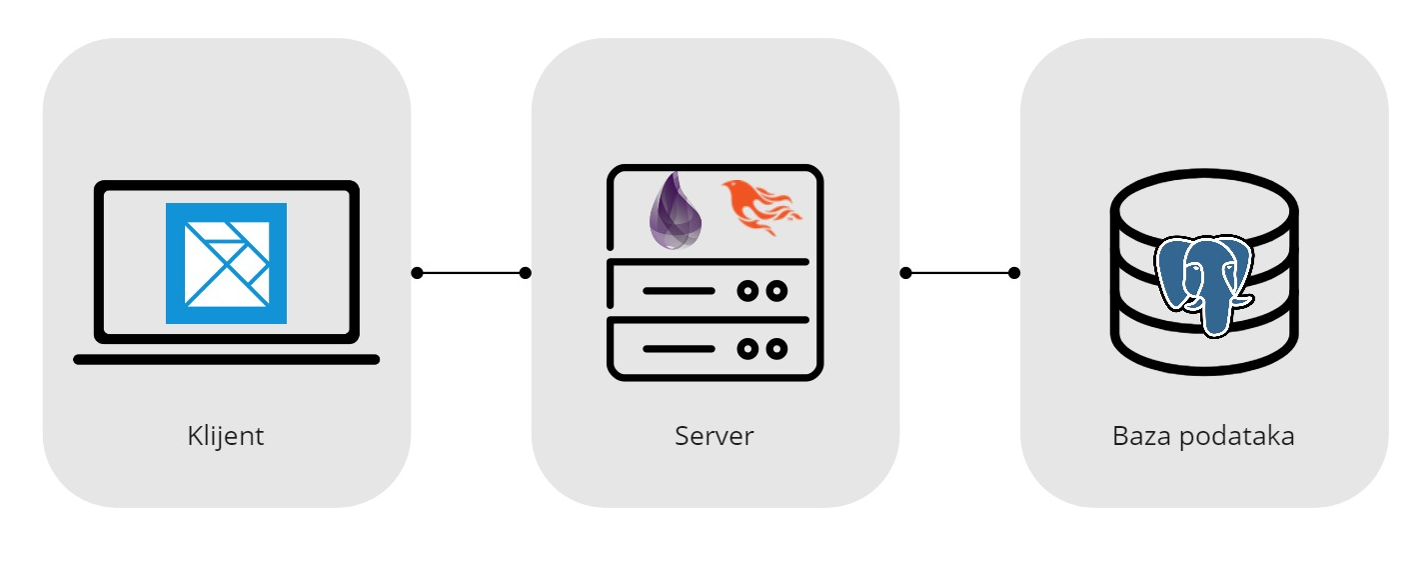
\includegraphics[width=0.9\textwidth]{msnr-arch.png}
  \caption{Arhitektura Portala MSNR \cite{rad}}
\end{figure}

\subsubsection{Struktura serverske strane portala}
\par U programskom jeziku Elixir, za razvoj veb aplikacija koristi se razvojni okvir \emph{Phoenix} \cite{phx}. Zasnovan je na obrascu \emph{model-pogled-upravljač} (eng. \emph{Model-View-Controller pattern, MVC}). Serverski deo aplikacija MSNR portal implementiran je kao \emph{Phoenix} projekat. Preciznije, projekat je u osnovi \emph{Mix} projekat, sa \emph{Phoenix} proširenjima. \emph{Mix} je osnovni alat ovog jezika koji se koristi za kreiranje, prevođenje i testiranje projekata. Pored ovog alata, potrebno je prethodno instalirati i menadžer paketa za ekosistem \emph{Erlang} pod nazivom \emph{Hex} \cite{hex}. Pri kreiranju \emph{Phoenix} projekta, dodeljeno mu je ime \emph{msnr{\textunderscore}api}. Na slici \ref{fig:msnr-str} je prikazana struktura projekta nakon uspešnog pokretanja komande za kreiranje. 

\begin{figure}[!ht]
  \centering
  \label{fig:msnr-str}
  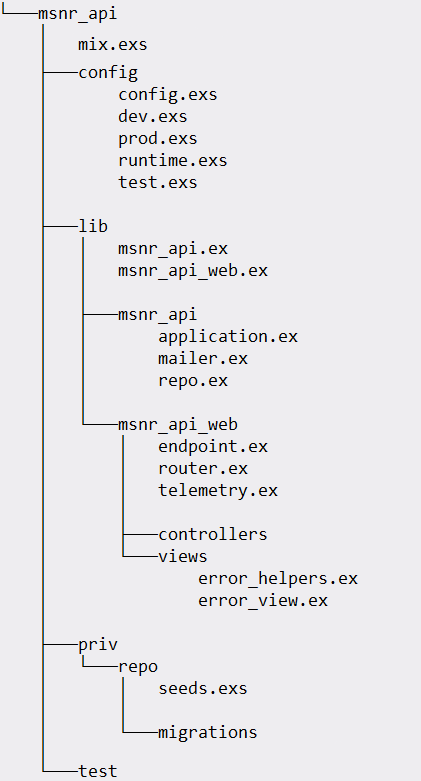
\includegraphics[width=0.5\textwidth]{msnr-str.png}
  \caption{Struktura \emph{Phoenix} projekta \emph{msnr{\textunderscore}api} \cite{rad}}
\end{figure}

\par U direktorijumu \emph{lib} nalaze se dva konteksta (eng. \emph{context}), tj. dva modula, od kojih svaki grupiše funkcije sa zajedničkom svrhom. Prvi kontekst je \emph{MsnrApi}, unutar koga je enkapsulirana sva domenska i poslovna logika, i definisani svi entiteti i funkcije za rad sa njima. Inicijalno su kreirana tri podmodula ovog konteksta: \emph{MsnrApi.Application}, koji pokreće aplikaciju, \emph{MsnrApi.Repo}, koji je zadužen za komunikaciju sa bazom, i \emph{MsnrApi.Mailer}, koji služi za slanje elektronske pošte. Drugi kontekst ima naziv \emph{MsnrApiWeb}, i on sadrži implementaciju za poglede i upravljače unutar arhitekture MVC. Njegovi podmoduli \emph{MnsrApiWeb.Endpoint} i \emph{MsnrApiWeb.Router} imaju ulogu u pripremi HTTP zahteva i njihovom prosleđivanju odgovarajućim upravljačima. 
\par Za sve obrade HTTP zahteva koristi se biblioteka \emph{Plug} \cite{plug}. Utikač (eng. \emph{plug}) je funkcija koja ima kao ulaznu i povratnu vrednost strukturu \emph{Plug.Conn} koja sadrži sve informacije o primljenom HTTP zahtevu. \emph{Phoenix} poziva utikače jedan za drugim, i svaki od njih transformiše ovu strukturu dok se obrada zahteva ne završi, i na kraju odgovor pošalje korisniku. Sa utikačima se povezuje veb server pod nazivom \emph{Cowboy}, a u mix.exs je automatski ubačena zavisnost \emph{plug{\textunderscore}cowboy}.
\par Kada se kreira novi \emph{mix} projekat, pored konfiguracione datoteke \emph{mix.exs}, i direktorijuma \emph{lib} koji sadrži osnovni k$\hat{o}$d aplikacije, kreira se i direktorijum \emph{test}. Unutar ovog direktorijuma će biti smešteni svi testovi vezani za serversku stranu aplikacije. 

\subsubsection{Struktura klijentske strane portala}
\par Klijent aplikacija Portala MSNR predstavlja jedan Elm projekat. Inicijalizacija ovog projekta podrazumeva kreiranje jednog praznog direktorijuma src i datoteke elm.json, a sam korisnik odlučuje o organizaciji datoteka unutar projekta. Na slici \ref{fig:msnr-elm} prikazano je rešenje organizacije Elm datoteka u okviru aplikacije Portal MSNR. 

\begin{figure}[!ht]
  \centering
  \label{fig:msnr-elm}
  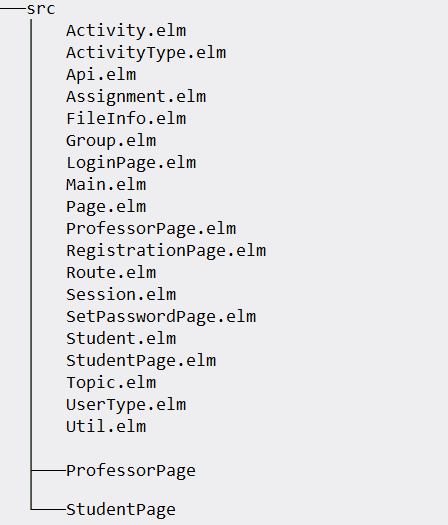
\includegraphics[width=0.6\textwidth]{msnr-elm.png}
  \caption{Struktura \emph{Elm} projekta \emph{msnr{\textunderscore}elm} \cite{rad}}
\end{figure}

\par U korenu projekta se nalazi osnovna datoteka \emph{Main.elm}, koja sadrži funkciju \emph{main} sa definicijom Elm aplikacije. Ostale datoteke sadrže definicije osnovnih stranica, entiteta, putanja i modula za komunikaciju sa serverom. U posebnim direktorijumima, izdvojene su datoteke za prikazivanje studentskih i profesorskih stranica. 
\par Korisnički interfejs portala implementiran je pomoću četiri funkcije: \emph{sandbox, element, document, application}. Ove funkcije se nalaze unutar modula \emph{Browser}, koji je deo paketa čija je uloga kreiranje Elm programa u pretraživaču. Funkcija \emph{sandbox} omogućava bazičnu interakciju sa korisnicima, bez komunikacije sa spoljnim svetom. Tu komunikaciju omogućava funkcija \emph{element}, pomoću koncepta komande, supskripcije, portova i oznaka (eng. \emph{flags}). Funkcija \emph{document} proširuje prethodnu funkciju tako što upravlja celim dokumentom i pruža kontrolu nad HTML elementima naslova i tela. Funkcija \emph{application} kreira aplikaciju koja upravlja url promenama. 
\par Aplikacija je kompajlirana tako da se kreira datoteka \emph{app.js}, koja se uključuje dokument \emph{index.html}. Pokreće se pozivanjem \emph{init} funkcije iz modula \emph{Main} i tada se vrši prosleđivanje putanje ka veb interfejsu preko oznaka. 
\par Elm aplikacija podeljena je na tri osnovna dela: stranice koje se koriste za prijavljivanje i registraciju korisnika, studentsku stranicu, i profesorske stranice. Pored njih, postoje i stranice koje nisu izdvojene u posebne module --- početna stranica i stranica koja se prikazuje u slučaju pogrešne putanje.


\section{Testiranje portala}
\par Testiranje ovakve aplikacije podrazumeva podelu na različite vrste testova. Za početak, jedinični testovi koji se odnose na individualne funkcije i upravljače koji barataju zahtevima u okviru serverskog dela aplikacije moraju biti napisani u programskom jeziku Elixir. Na serverskoj strani, potrebno je napisati i testove koji simuliraju zahteve API-ju i verifikuju odgovore od baze. Sa druge strane, jedinični testovi koji se fokusiraju na pojedinačne komponente i funkcije korisničkog interfejsa moraju biti napisani u programskom jeziku Elm. Nakon pojedinačnog testiranja klijentske i serverske aplikacije, slede integracioni testovi koji proveravaju kako korisnički interfejs funkcioniše zajedno sa API-jem. Na kraju je neophodno testirati celokupan sistem, od korisničkog interfejsa do baze podataka, pisanjem sistemskih testova. S obzirom na to da se radi o veb aplikaciji, mogu se sprovesti i testovi opterećenja koji će proveriti kako portal podnosi velike količine zahteva i korisnika. 
%U narednim poglavljima biće detaljno prikazano sprovođenje svih ovih testova.

\chapter{Testiranje serverskog dela aplikacije}
\label{chp:elixir}

\par U ovom poglavlju biće predstavljeni različiti koncepti testiranja u programskom jeziku Elixir, kroz pisanje testova za serverski deo aplikacije Portal MSNR. \textit{ExUnit} je Elixir-ov ugrađeni razvojni okvir koji ima sve što je neophodno za iscrpno testiranje koda i biće osnova za sve testove kroz ovo poglavlje \cite{exunit}.

\section{Testiranje jedinica koda u programskom jeziku Elixir}
\label{sec:elixunit}

\par S obzirom na to da je Elixir funkcionalni jezik, može se diskutovati o tome šta se smatra "jedinicom". Uobičajeno je da se jedinični testovi fokusiraju na pojedinačnu funkciju i njenu logiku, kako bi se opseg testa održavao što užim, radi bržeg pronalaženja grešaka. Međutim, nekada ima smisla da se u opseg testa uključi više modula ili procesa, i time se proširi definicija jedinice koda i olakša održavanje samih testova. 
\par Pisanje testova u programskom jeziku Elixir je moguće bez potrebe za drugim bibliotekama, jer je \emph{ExUnit} razvijan zajedno sa samim jezikom od početka. Svi testovi su implementirani kao Elixir skripte, pa je pri davanju imena testu neophodno koristiti ekstenziju datoteke \emph{.exs}. Pre pokretanja testova potrebno je pokrenuti \emph{ExUnit}, kao što je prikazano u primeru koda \ref{lst:start}. Ova naredba se obično navodi unutar automatski generisane datoteke \emph{test/test{\textunderscore}helper.exs}. 

\begin{lstlisting}[language=elixir, caption={Pokretanje ExUnit},captionpos=b, label={lst:start}]
# test/test_helper.exs

ExUnit.start()
\end{lstlisting}

\par Testovi se pokreću najpre pozicioniranjem u direktorijum projekta, a zatim navođenjem komande \emph{mix test}. Ova komanda pokreće sve testove koji se nalaze unutar \emph{test} direktorijuma. Navođenjem parametra \emph{--only} i imena testa ili modula može se pokrenuti specifičan test ili skup testova unutar jednog modula. Pozivanje naredbe \emph{mix test} pokreće sve testove, i daje sledeći izlaz:  

\begin{lstlisting}[style=DOS]
PS C:\Users\panap\testing-msnr-portal\portal\msnr_api> mix test

..............
Finished in 0.2 seconds (0.00s async, 0.2s sync)
16 tests, 0 failures
\end{lstlisting}

\par Svita testova (eng. \emph{test suite}) je kolekcija testova slučajeva upotrebe, koji imaju isti posao, ali različite scenarije. Ona može služiti kao dokumentacija, sa opisima o očekivanom ponašanju koda, tako da treba voditi računa da bude dobro organizovana. \emph{ExUnit} dolazi sa veoma korisnim funkcijima i makroima koji omogućavaju tu organizaciju u jednu čitljivu i održivu datoteku. Alat \emph{describe} omogućava davanje opisa grupe testova, kao i dodeljivanja zajedničke pripreme podataka za celu grupu. Preporuka je za početak grupisati testove po funkciji, kao što je prikazano u primeru koda \ref{lst:desc}, ali odluka o načinu grupisanja je na pojedincu. Svrha je čitljivost i lakše razumevanje. \par Testovi u Elixir projektima se organizuju u module i test slučajeve. U ovom primeru, modul pod nazivom \emph{AccountsTest} sadrži testove koji se odnose na kontekst koji opisuje korisnike. Blok \emph{describe} iz primera se sastoji od dva test slučaja, i odnosi se na funkciju \emph{get{\textunderscore}user}, koja vrši jednostavno dohvatanje korisnika iz baze prosleđivanjem identifikatora. Navođenjem ključne reči \emph{test}, a za njom niske koja treba da opiše šta je to što test treba da uradi, definiše se jedna funkcija koja predstavlja test slučaj. Na primeru \emph{describe} bloka funkcije \emph{get{\textunderscore}user}, prikazana su dva test slučaja, od kojih jedan proverava uspešno izvršavanje funkcije kada se prosledi validan identifikator, a drugi proverava da li se javlja greška kada se prosledi identifikator korisnika koji ne postoji.
\par Unutar jednog test slučaja poziva se funkcija ili upravljač i proverava se očekivani rezultat. Makroom \emph{assert} se testira da li je izraz istinit. U slučaju da nije, test ne prolazi i izbacuje grešku. Ako funkcija \emph{get{\textunderscore}user} vrati korisnika koji je jednak postojećem korisniku iz baze, ovaj test uspešno prolazi.

\begin{lstlisting}[language=elixir, caption={Opisivanje testova unutar jedne grupe, na primeru funkcije za dohvatanje korisnika},captionpos=b, label={lst:desc}]
defmodule MsnrApi.Queries.AccountsTest  do
...
describe "get_user/1" do
    test "success: it returns a user when given a valid id" do
      existing_user = Factory.insert(:user)
      assert returned_user = Accounts.get_user!(existing_user.id)
      assert returned_user == existing_user
    end

    test "error: it returns a NoResultsError when a user doesn't exist" do
      assert_raise Ecto.NoResultsError, fn ->
        Accounts.get_user!(invalid_id) end
    end
 end
\end{lstlisting}


\par U slučaju da leva i desna strana izraza navedenog nakon makroa \emph{assert} nisu jednake, test ne prolazi, a \emph{ExUnit} daje obaveštenje o tome koji od testova su neuspešni, kao i koje su prava i očekivana vrednost. Izlaz koji se dobije u slučaju da dohvaćeni korisnik nije onaj koji je očekivan, prikazan je na listingu \ref{lst:term}. 

\begin{lstlisting}[style=DOS, caption={Izlaz u slučaju testa koji ne prolazi},captionpos=b, label={lst:term}]
1) test get_user/1 success: it returns a user when given a valid id (MsnrApi.Queries.AccountsTest)
     test/msnr_api/queries/accounts_test.exs:73
     ** (Ecto.NoResultsError) expected at least one result but got none in query:

     from u0 in MsnrApi.Accounts.User,
       where: u0.id == ^6

     code: assert returned_user = Accounts.get_user!(6)
     stacktrace:
       (ecto 3.7.1) lib/ecto/repo/queryable.ex:156: Ecto.Repo.Queryable.one!/3
       test/msnr_api/queries/accounts_test.exs:76: (test)

Finished in 0.5 seconds (0.00s async, 0.5s sync)

2 tests, 1 failures
\end{lstlisting}


\par U narednoj listi dati su nazivi i opisi makroa koji se mogu koristiti u testovima pored makroa \emph{assert}: 
 \begin{itemize}
 \item \emph{refute} --- koristi se kada je potrebno utvrditi da je izraz uvek neistinit. 
 \item \emph {assert{\textunderscore}raise} --- koristi se kada je potrebno proveriti da li se javlja konkretan izuzetak.
 \item \emph{assert{\textunderscore}receive} --- koristi se kada je potrebno proveriti da li je proces primio konkretnu poruku.
 \item \emph {capture{\textunderscore}io} --- koristi se kada je potrebno proveriti da li se na standardanom izlazu ispisuje očekivano.
 \item \emph{capture{\textunderscore}log} --- koristi se kada je potrebno proveriti sadržaj log poruka, npr. pri pozivu \emph{Logger.info}.
 \item \emph{setup i setup{\textunderscore}all} --- koriste se kada je potrebno izvršiti pripremu testova, pokreću se pre svakog testa, ili pre jedne grupe.
 \end{itemize}
 
\par U test slučaju greške iz primera \ref{lst:desc}, iskorišćen je i makro \emph{assert{\textunderscore}raise} --- očekuje se da se pri dohvatanju korisnika koji ne postoji javi izuzetak \emph{NoResultsError}. Upotreba makroa \emph{refute} i \emph{setup} prikazana je u primeru dela koda \ref{lst:del}. K$\hat{o}$d  unutar makroa \emph{setup} će se pokretati pre svakog testa, a u ovom primeru priprema podrazumeva eksplicitno dohvatanje konekcije sa bazom podataka pre izvršavanja svakog od testova. Pri testiranju funkcije \emph{delete{\textunderscore}user}, koja treba da ukloni korisnika iz baze, iskorišćen je makro \emph{refute}. Kada se pokuša dohvatanje korisnika koji je prethodno izbrisan, trebalo bi da to nije moguće i da dođe do greške. Zbog toga je u ovom slučaju \emph{refute} dobar izbor.
 
\begin{lstlisting}[language=elixir, caption={Upotreba makroa \emph{setup} i \emph{refute} na primeru funkcije \emph{delete{\textunderscore}user}},captionpos=b, label={lst:del}]
setup do
    Ecto.Adapters.SQL.Sandbox.checkout(MsnrApi.Repo)
end
  
describe "delete_user/1" do
   test "success: it deletes the user" do
      user = Factory.insert(:user)
      assert {:ok, _deleted_user} = Accounts.delete_user(user)

      refute Repo.get(User, user.id)
   end
end
\end{lstlisting}

\section{Integraciono testiranje}
\label{sec:elixint}\}
\par Nakon dobro istestiranih pojedinačnih funkcija i modula, potrebno je proveriti da li komponente funkcionišu ispravno kao celina. U ovoj sekciji biće prikazani testovi koji proveravaju da li različiti delovi sistema koji komuniciraju međusobno, kao i sa nekim eksternim sistemima, rade to na ispravan način.

\subsection{Testiranje komunikacije sa bazom podataka}
\par \emph{Ecto} biblioteka zadužena je za sve interakcije sa relacionim bazama podataka u \emph{Elixir} okruženju \cite{ecto}. Pored komunikacije sa bazom, \emph{Ecto} ima i ulogu u validaciji. Moduli ove biblioteke koje je značajno naglasiti su: \emph{Ecto.Repo}, \emph{Ecto.Schema} i \emph{Ecto.Changeset}. \emph{Ecto.Repo} opisuje gde se nalaze podaci, odnosno definiše omotač oko baze preko kog se ostvaraje komunikacija sa bazom. \emph{Ecto.Schema} ima ulogu u definisanju mapiranja eksternih podataka u \emph{Elixir} strukture. Koncept skupa promena (eng. \emph{changeset}) odnosi se na proces validacije podataka, njihovog konvertovanja i provere dodatnih uslova pre nego što se upišu u bazu. \emph{Ecto.Changeset} modul opisuje kako se menjaju podaci. U ovom delu, prikazani su testovi koji proveravaju da li k$\hat{o}$d koristi funkcionalnosti \emph{Ecto} biblioteke na ispravan način.
\par \emph{Ecto} i svi potrebni moduli se podrazumevano uključuju prilikom kreiranja \emph{Phoenix} projekta. Pre samog pisanja testova, neophodno je podesiti sve parametre za komunikaciju sa bazom podataka \emph{PostgreSQL} u testnom okruženju. U datoteci \emph{config/test.exs} potrebno je uneti podatke kao što je prikazano u primeru koda \ref{lst:conf}. Pokretanjem naredbe \emph{MIX{\textunderscore}ENV=test mix ecto.create} iz komandne linije, lokalno će se kreirati \emph{msnr{\textunderscore}api{\textunderscore}test} baza podataka.

\begin{lstlisting}[language=elixir, caption={Konfiguracija baze podataka u testnom okruženju},captionpos=b, label={lst:conf}]
  config :msnr_api, MsnrApi.Repo,
  username: "postgres",
  password: "1234",
  database: "msnr_api_test#{System.get_env("MIX_TEST_PARTITION")}",
  hostname: "localhost",
  pool: Ecto.Adapters.SQL.Sandbox,
  pool_size: 10
\end{lstlisting}

\par Svi testovi u vezi sa bazom podataka nalaze se u direktorijumima \textit{'/test/msnr{\textunderscore}api/schema'} i \textit{'/test/msnr{\textunderscore}api/queries'}, u okviru projekta \emph{msnr{\textunderscore}api}. 
\par Na početku, napisani su jednostavni testovi koji proveravaju ispravnost definisanja struktura pomoću \emph{Ecto.Schema} modula. Primer definisanja entiteta dodeljenih aktivnosti  dat je u primeru koda \ref{lst:schema}. Pomoću makroa \emph{schema} i \emph{field} definišu se tabele, njihova polja i relacije sa drugim tabelama. Oni istovremeno definišu i Elixir strukturu --- u ovom primeru, ta struktura se naziva \emph{Assignment}. Pored ovog, i svi ostali entiteti su definisani kao konteksti u okviru konteksta \emph{MsnrApi}, koji sadrži domensku logiku aplikacije. Funkcija \emph{changeset/2} biće objašnjena kasnije.

\begin{lstlisting}[language=elixir, caption={Shema tabele assignments},captionpos=b, label={lst:schema}]
defmodule MsnrApi.Assignments.Assignment do
  use Ecto.Schema
  import Ecto.Changeset

  schema "assignments" do
    field :comment, :string
    field :completed, :boolean, default: false
    field :grade, :integer
    field :student_id, :id
    field :group_id, :id
    field :activity_id, :id
    field :related_topic_id, :id
    timestamps()
  end

  def changeset(assignment, attrs) do
    assignment
    |> cast(attrs, [:comment, :grade])
    |> validate_required([:comment, :grade])
  end
...
\end{lstlisting}

\subsubsection{Testiranje polja i tipova}
\par Test koji se odnosi na prethodni primer prikazan je u kodu \ref{lst:testschema}. Ovo je primer jednostavnog jediničnog testa koji proverava da li definisana shema ima tačna polja i odgovarajuće tipove. Unutar testa se prvo prolaskom kroz sva polja Assignment strukture izvuku polje i njegov tip, i zatim se navodi ključna reč \emph{assert}, kojom se proverava da li su prava polja i tipovi jednaki očekivanim. Lista \emph{@expected{\textunderscore}fields{\textunderscore}with{\textunderscore}types} definisana je kao lista parova polja i odgovarajućih tipova, kao što su navedeni u primeru \ref{lst:schema}. Unutar \emph{assert} naredbe, i prava i očekivana lista pretvorene su u \emph{MapSet} strukturu, kako bi se redosledi polja poklapali sa obe strane. Slični testovi napisani su i za sve ostale entitete navedene u sekciji \ref{sec:entiteti}.

\begin{lstlisting}[language=elixir, caption={Test za proveru polja i tipova tabele \emph{assignments}},captionpos=b, label={lst:testschema}]
defmodule MsnrApi.Schema.AssignmentTest do
...  
  describe "fields and types" do
    test "it has the correct fields and types" do
      actual_fields_with_types =
        for field <- Assignment.__schema__(:fields) do
          type = Assignment.__schema__(:type, field)
          {field, type}
         end
    
      assert MapSet.new(actual_fields_with_types) == MapSet.new(@expected_fields_with_types)
  end
 end
\end{lstlisting}

\subsubsection{Testiranje skupa promena}
\par Funkcija \emph{changeset} iz primera koda \ref{lst:schema} obuhvata različite transformacije podataka, kao i njihovu validaciju pre unosa u bazu podataka. Svrha ove funkcije je da svi podaci koji se unose ili ažuriraju u bazi budu ispravni i u skladu sa zahtevima aplikacije. Svaka od shema ima svoju definiciju polja i svoju \emph{changeset} funkciju. Tokom razvoja aplikacije, shemama se mogu dodavati različite izmene, kao što su nova polja, ili izmene u samim validacijama unutar funkcije \emph{changeset}. Funkcija \emph{cast} je prva u nizu funkcija koje se pozivaju i ona ograničava polja koja se mogu menjati. U slučaju modula \emph{Assignment}, to su polja \emph{comment} i \emph{grade}. Funkcija validaterequired proverava obavezna polja. Rezultat izvršavanja ovih funkcija je takođe \emph{Ecto.Changeset} struktura, koja sadrži informacije o promenama koje treba izvršiti, validnost izmena i greške validacije ukoliko one postoje.
\par Testovi koji se odnose na ove funkcije implementirani su unutar \emph{describe} bloka \emph{''changeset/2''}, za svaki od entiteta aplikacije. Oni pokrivaju i uspešan scenario, i neke od slučajeva greški. Koji od ovih scenarija će se desiti, zavisi od ispravnosti prosleđenih parametara funkcije. Parametri koji će se prosleđivati u testovima formirani su unutar pomoćnih funkcija koje se nalaze u modulu \emph{SchemaCase}. On se nalazi u direktorijumu \emph{msnr{\textunderscore}api/test/support}, zajedno sa ostalim datotekama koje sadrže zajednički k$\hat{o}$d. Da bi ova datoteka bila prepoznata kada se pokreću testovi, potrebno je dodati dve linije unutar \emph{mix.exs} datoteke, koje su prikazane u kodu \ref{lst:mst}. Ovime se govori aplikaciji da uključi sve datoteke u \emph{test} direktorijumu prilikom kompilacije u testnom okruženju. Tako \emph{SchemaCase} postaje dostupan isključivo prilikom testiranja.

\begin{lstlisting}[language=elixir, caption={Uključivanje datoteka iz test direktorijuma pri kompilaciji u testnom okruženju},captionpos=b, label={lst:mst}]
defp elixirc_paths(:test), do: [''lib'', ''test'']
defp elixirc_paths(_), do :[''lib'']
...
def project do [
     ...
     elixirc_paths: elixirc_paths(Mix.env()), 
]
\end{lstlisting}

\par Modul \emph{SchemaCase} sadrži dve funkcije, od kojih jedna konstruiše realistične podatke ispravnih tipova, a druga konstruiše podatke koji su pogrešnog tipa u odnosu na polje tabele. Funkcije \emph{valid{\textunderscore}params} i \emph{invalid{\textunderscore}params} prikazane su u primeru koda \ref{lst:faker}. Ove funkcije kao povratnu vrednost imaju mapu koja sadrži niske naziva polja kao ključeve, i odgovarajuće generisane vrednosti koje njima odgovaraju. Biblioteka \emph{Faker} \cite{faker} ima ulogu u formiranju nasumičnih realističnih podataka. Na primer, pomoću modula ove biblioteke pod nazivom \emph{Lorem}, mogu se dobiti nasumične reči koje će predstavljati polja tabela koja treba da imaju nisku kao svoju vrednost. \emph{Faker} je potrebno uključiti u zavisnosti projekta, dodavanjem linije \textit{\{:faker, ''$\sim$> 0.17'', only: :test\}} u \emph{deps} delu konfiguracione datoteke \emph{mix.exs}. Biblioteku nije potrebno koristiti u razvojnom i produkcionom okruženju, te se ovom linijom ograničava njena upotreba samo na testno okruženje.

\begin{lstlisting}[language=elixir, caption={Definicije pomoćnih funkcija \emph{valid{\textunderscore}params} i \emph{invalid{\textunderscore}params}},captionpos=b, label={lst:faker}]

def valid_params(fields_with_types) do

    valid_value_by_type = %{
      string: fn -> Faker.Lorem.word() end,
      naive_datetime: fn -> Faker.NaiveDateTime.backward(Enum.random(0..100)) end,
      id: fn -> Enum.random(0..100) end,
      ... 
    }

    for {field, type} <- fields_with_types, into: %{} do
      case field do
        {Atom.to_string(field), valid_value_by_type[type].()}
      end
    end
  end

  def invalid_params(fields_with_types) do
    invalid_value_by_type = %{
      string: fn -> DateTime.utc_now() end,
      naive_datetime: fn -> Faker.Lorem.word() end,
      id: fn -> DateTime.utc_now() end,
      ...
    }

    for {field, type} <- fields_with_types, into: %{} do
      {Atom.to_string(field), invalid_value_by_type[type].()}
    end
  end

\end{lstlisting}


\par Funkcija \emph{changeset/2} iz primera koda \ref{lst:schema}, koja kao argumente prihvata strukturu \emph{Assignment} i listu atributa, ima ulogu da validira prisustvo dva polja u tabeli \emph{assignments} --- polja \emph{comment} i \emph{grade}. Test slučaj koji proverava uspešnu putanju izvršavanja funkcije \emph{changeset/2} prikazan je u primeru koda \ref{lst:changeset}. Funkciji se prosleđuju validni parametri, kreirani pomoću prethodno definisane funkcije \emph{valid{\textunderscore}params}. Nakon toga, proverava se da li je dobijeni skup promena validan, a onda se pojedinačno za svako neophodno polje proverava da li je ispravno.

\begin{lstlisting}[language=elixir, caption={Test slučaj uspešne upotrebe funkcije \emph{changeset/2}},captionpos=b, label={lst:changeset}]
  test "success: returns a valid changeset when given valid arguments" do
      valid_params = valid_params(@required_fields)
      changeset = Assignment.changeset(%Assignment{}, valid_params)

      assert %Changeset{valid?: true, changes: changes} = changeset

      for {field, _} <- @required_fields do
        actual = Map.get(changes, field)
        expected = valid_params[Atom.to_string(field)]
        assert actual == expected,
          "Values did not match for: #{field}\nexpected: #{inspect(expected)}\nactual: #{inspect(actual)}"
      end
  end 
\end{lstlisting}

\par Drugi test slučaj koji je potrebno pokriti je slučaj kada dolazi do greške zbog prosleđenih parametara koji nisu ispravni. Funkciji \emph{changeset} se proslede parametri formirani pomoću funkcije \emph{invalid{\textunderscore}params}, i očekuje se da će dobijeni skup promena biti nevalidan. Nakon te provere, proverava se lista grešaka, koja bi trebalo da sadrži svako od neophodnih polja. Pošto su prosleđeni parametri pogrešnog tipa, koji se ne može kastovati u odgovarajući ispravni tip, očekuje se da u okviru greške, vrsta validacije bude \emph{:cast}, pa se i to na kraju proverava još jednom \emph{assert} naredbom. Ovaj test slučaj prikazan je u primeru koda \ref{lst:cast}. 

\begin{lstlisting}[language=elixir, caption={Test slučaj neuspešne upotrebe funkcije \emph{changeset/2}, prosleđivanjem nekastabilnih parametara},captionpos=b, label={lst:cast}]
test "error: returns an invalid changeset when given uncastable values" do
      invalid_params = invalid_params(@required_fields)

      assert %Changeset{valid?: false, errors: errors} = Assignment.changeset(%Assignment{}, invalid_params)

      for {field, _} <- @required_fields do
        assert errors[field], "the field: #{field} is missing from errors."

        {_, meta} = errors[field]
        assert meta[:validation] == :cast,
          "The validation type #{meta[:validation]} is incorrect."
      end
end
\end{lstlisting}

\par Ako se funkciji \emph{changeset} prosledi prazna mapa, tj. ako nedostaju polja koja inače moraju biti navedena, javlja se greška čiji je tip validacije \emph{:required}. Primer ovog test slučaja dat je u kodu \ref{lst:req}. U ovom slučaju, nakon provere da li je skup promena neispravan, proverava se da li je svako od zahtevanih polja u listi grešaka, a nakon toga i da li je tip validacije \emph{:required}. Na kraju, pomoću \emph{refute} naredbe, utvrđuje se da se opciona polja ne nalaze u listi grešaka. To su polja koja nije neophodno navesti pri pozivanju ove funkcije, i oni se zato ne trebaju naći ni među greškama.

\begin{lstlisting}[language=elixir, caption={Test slučaj neuspešne upotrebe funkcije \emph{changeset/2}, sa nedostajućim parametrima},captionpos=b, label={lst:req}]
test "error: returns an error changeset when required fields are missing" do
      params = %{}
      assert %Changeset{valid?: false, errors: errors} = Assignment.changeset(%Assignment{}, params)

      for {field, _} <- @required_fields do
        assert errors[field], "The field #{field} is missing from errors."
        {_, meta} = errors[field]
        assert meta[:validation] == :required,
        "The validation type #{meta[:validation]} is incorrect."
      end

      for field <- @optional_fields do
        refute errors[field], "The optional field #{field} is required when it shouldn't be."
      end
end
\end{lstlisting}

\par Neke od shema će unutar svoje \emph{changeset} funkcije imati i dodatne validacije, kao što je na primer validacija jedinstvenih polja. Na primeru sheme \emph{users}, nakon ostalih izmena i validacija, dodat je i sledeći poziv funkcije: \emph{unique{\textunderscore}constraint(:email)}. Ova funkcija obaveštava \emph{Ecto} da u tabeli korisnika ne sme postojati dva korisnika sa istom imejl adresom, tj. polje \emph{:email} mora biti jedinstveno za svakog korisnika. Ako se desi pokušaj registrovanja korisnika sa već iskorišćenom imejl adresom, dolazi do greške tipa \emph{:unique}. Ovaj test slučaj prikazan je u primeru koda \ref{lst:uniq}. Neophodno je ostvariti direktan pristup bazi podataka, pa je prva linija unutar test slučaja naredba kojom se kreira konekcija sa bazom. Zatim se u bazu ubacuje novi korisnik (pozivom \emph{MsnrApi.Repo.insert()}), i time je završena priprema testa. Nakon toga, pokušava se ubacivanje još jednog korisnika sa istom imejl adresom. To bi trebalo da izazove grešku, što se proverava prvom \emph{assert} naredbom. Druga \emph{assert} naredba proverava da li se greška odnosi na polje \emph{:email}, a treća utvrđuje i tačnu vrstu greške, slično kao u prethodnim primerima. Za razliku od prethodnih testova, meta podaci u ovom slučaju nisu validacija, već ograničenje (eng. \emph{constraint}). 

\begin{lstlisting}[language=elixir, caption={Test slučaj neuspešne upotrebe funkcije \emph{changeset/2}, pri narušavanju ograničenja jedinstvenosti},captionpos=b, label={lst:uniq}]
test "error: returns an error changeset when an email is reused" do
      Ecto.Adapters.SQL.Sandbox.checkout(MsnrApi.Repo)

      {:ok, existing_user} =
        %User{}
        |> User.changeset(valid_params(@required_fields))
        |> MsnrApi.Repo.insert()
        
      changeset_with_reused_email =
        %User{}
        |> User.changeset(valid_params(@required_fields)
        |> Map.put("email", existing_user.email))

      assert {:error, %Changeset{valid?: false, errors: errors}} =
        MsnrApi.Repo.insert(changeset_with_reused_email)

      assert errors[:email], "The field :email is missing from errors."
      {_, meta} = errors[:email]

      assert meta[:constraint] == :unique,
      "The validation type #{meta[:validation]} is incorrect."
    end
\end{lstlisting}

\par Što se tiče faze rušenja, \emph{Ecto} obezbeđuje da svaki pojedinačni test ne mora da prati i vraća okruženje na prvobitno stanje. Za to je zadužen \emph{Ecto.Sandbox}, koji omogućava paralelno izvršavanje testova bez deljenog stanja u bazi podataka i automatski vrši poništavanje svih promena u bazi na kraju svakog testa. Konfiguracija je prikazana u primeru koda \ref{lst:sand}. U datoteci schema{\textunderscore}case potrebno je dodati \emph{setup} blok koji će svi testovi koji koriste ovaj obrazac pokretati na početku izvršavanja. Manuelni režim podrazumeva da će svaki test moći da zahteva svoju \emph{Sandbox} konekciju. Takođe, u konfiguracionoj datoteci \emph{config/test.exs}, u \emph{Ecto} delu, dodaju se linije koje obaveštavaju \emph{Ecto} da će se koristiti \emph{Sandbox}.
%TODO sta je connection pool?? kako prevesti
\begin{lstlisting}[language=elixir, caption={Podešavanje \emph{Ecto.Sandbox}},captionpos=b, label={lst:sand}]

# msnr_api/test/schema_case.ex
setup do
    Ecto.Adapters.SQL.Sandbox.mode(MsnrApi.Repo, :manual)
end
...
# msnr_api/config/test.exs
config :msnr_api, MsnrApi.Repo,
  database: "msnr_api_test",
  pool: Ecto.Adapters.SQL.Sandbox,
\end{lstlisting}


\subsubsection{Testiranje upita}
\par U ovom delu biće prikazano kako su testirani konteksti entiteta. Modul koji će služiti kao primer se odnosi na korisnike --- \emph{MsnrApi.Accounts}. Struktura jednog dela ove datoteke prikazana je u primeru koda \ref{lst:act}, gde se može videti upotreba funkcija za interakciju sa bazom podataka kroz modul \emph{Ecto.Repo}. Prikazane su osnovne operacije dohvatanja redova iz tabele, dodavanja novog reda, ažuriranja reda, i brisanja reda iz zadate tabele. Unutar funkcija \emph{create{\textunderscore}user} i \emph{update{\textunderscore}user} poziva se i funkcija \emph{User.changeset}, koja je već prethodno istestirana.  

\begin{lstlisting}[language=elixir, caption={Definicija modula \emph{MsnrApi.Accounts}},captionpos=b, label={lst:act}]
defmodule MsnrApi.Accounts do
  alias MsnrApi.Repo
  alias MsnrApi.Accounts.User

 def list_users do
    Repo.all(User)
  end
  
  def get_user!(id), do: Repo.get!(User, id)

  def create_user(attrs \\ %{}) do
    %User{}
    |> User.changeset(attrs)
    |> Repo.insert()
  end

  def update_user(%User{} = user, attrs) do
    user
    |> User.changeset(attrs)
    |> Repo.update()
  end

  def delete_user(%User{} = user) do
    Repo.delete(user)
  end
\end{lstlisting}

\subsubsection{Fabrike za pripremu podataka}
\par Prilikom pisanja testova koji pristupaju tabelama baze podataka, za dohvatanje podataka u fazi pripreme, pogodno je iskoristiti obrazac fabrike (eng. \emph{factory pattern}). Kako aplikacija raste, održavanje testova postaje zahtevnije, i u tome značajno pomaže imati jedan izvor za pripremu podataka. U slučaju testiranja interakcija sa bazom podataka, kreirana je zajednička datoteka \emph{msnr{\textunderscore}api/test/support/factory.ex}. Pored toga, kreiran je poseban direktorijum \emph{msnr{\textunderscore}api/test/support/factories} u kome će se nalaziti pojedinačne fabrike za svaki od entiteta. U osnovi ovih fabrika nalazi se biblioteka \emph{ExMachina} \cite{exmachina}. Ova biblioteka obezbeđuje podatake za sheme, kao i mehanizam za ubacivanje podataka u bazu bez pisanja koda. Kao prvi korak, \emph{ExMachina} je dodata kao zavisnost aplikacije: u okviru datoteke \emph{msnr{\textunderscore}api/mix.exs} ubačena je linija \textit{\{:exmachina, ''$\sim$> 2.7.0'', only: :test\}}. Da bi mogla da se koristi, pokrenuti komandu \emph{mix deps.get} iz komandne linije.
\par Datoteka \emph{factory.ex} prikazana je u primeru koda \ref{lst:fact}. Prva linija uključuje biblioteku \emph{ExMachina} i prosleđuje joj naziv repozitorijuma aplikacije, što znači da će ova fabrika moći da se koristi specifično u tom repozitorijumu. Ostatak datoteke su uključivanja pojedinačnih fabrika za svaki kontekst aplikacije. U okviru testova za te kontekste, importovaće se samo ova \emph{factory.ex} datoteka.

\begin{lstlisting}[language=elixir, caption={Definicija modula \emph{Factory}},captionpos=b, label={lst:fact}]
defmodule MsnrApi.Support.Factory do

  use ExMachina.Ecto, repo: MsnrApi.Repo
  use MsnrApi.UserFactory
  use MsnrApi.ActivityFactory
  use MsnrApi.ActivityTypeFactory
  use MsnrApi.AssignmentFactory
  use MsnrApi.DocumentFactory
  use MsnrApi.GroupFactory
  use MsnrApi.SemesterFactory
  use MsnrApi.StudentRegistrationFactory
  use MsnrApi.StudentFactory
  use MsnrApi.TopicFactory
end
\end{lstlisting}

\par Definicija funkcije fabrike data je u primeru koda \ref{lst:userfact}, u kome je prikazana definicija fabrike za korisnika. Po konvenciji biblioteke, pri imenovanju ovih funkcija neophodno je navesti ime sheme, i zatim \emph{''{\textunderscore}factory''}. Povratna vrednost funkcije je struktura sheme sa popunjenim lažnim vrednostima, dobijenim iz \emph{Faker} biblioteke. 

\begin{lstlisting}[language=elixir, caption={Definicija modula \emph{UserFactory}},captionpos=b, label={lst:userfact}]
defmodule MsnrApi.UserFactory do
  alias MsnrApi.Queries.AccountsTest
  alias MsnrApi.Accounts.User

  defmacro __using__(_opts) do
    quote do
      def user_factory do
        %User {
          email: Faker.Internet.email(),
          first_name: Faker.Person.first_name(),
          last_name: Faker.Person.last_name(),
         	...
        }
      end
 ...
\end{lstlisting}

\par U direktorijumu za pomoćne datoteke \emph{msnr{\textunderscore}test/support} kreiran je još jedan modul --- \emph{DataCase}. Ovaj modul služiće za sve situacije u kojima je potrebno baratati podacima pri interakciji sa bazom. Modul je prikazan u primeru koda \ref{lst:datacase}. U njemu se mogu nalaziti pomoćne funkcije koje će se koristiti u testovima, slično kao kod modula \emph{SchemaCase} koji je korišćen pri testiranju samih shema. U okviru datoteke, obezbeđena je zajednička priprema \emph{Sandbox} konekcija, i uključeni su aliasi za fabrike i za repozitorijum, koji će biti potrebni pri testiranju upita. Ako je neka funkcija fokusirana na pravljenju podataka, dobra je praksa smestiti je u fabriku. U suprotnom, pripadaće nekom ovakvom obrascu slučaja (eng. \emph{case template}), kao što je \emph{DataCase}. 

\begin{lstlisting}[language=elixir, caption={Definicija modula \emph{DataCase}},captionpos=b, label={lst:datacase}]
defmodule MsnrApi.Support.DataCase do

  use ExUnit.CaseTemplate

  using do
    quote do
      alias MsnrApi.{Support.Factory, Repo}
      alias Ecto.Changeset

      import Ecto.Query
      import MsnrApi.Support.DataCase
    end
  end

  setup _ do
    Ecto.Adapters.SQL.Sandbox.mode(MsnrApi.Repo, :manual)
  end
end
\end{lstlisting}

\subsubsection{Testiranje osnovnih CRUD operacija}

\par Datoteka \emph{MsnrApi.Accounts} sadrži osnovne operacije kreiranja, čitanja, ažuriranja i brisanja (eng. \emph{Create, Read/get, Update, Delete --- CRUD}) iz tabele. Testiranje ovih jednostavnih funkcija biće prikazano na primeru datoteke \emph{MsnrApi.Queries.AccountsTest}. U primeru koda \ref{lst:create} prikazani su testovi koji proveravaju ispravnost funkcije \emph{create{\textunderscore}user/1}. Prva linija unutar testa uspešne putanje koristi funkciju fabrike. Funkcija \emph{string{\textunderscore}params{\textunderscore}for} uzima atom \emph{:user} i sama poziva funkciju \emph{user{\textunderscore}factory}. \emph{ExMachina} obezbeđuje da povratna vrednost ove funkcije bude mapa sa ključevima koji su niske i predstavljaju parametre, koji se zatim prosleđuju funkciji \emph{create{\textunderscore}user} u fazi delovanja. S obzirom na to da je pozivom te funkcije izvršen upis u bazu, u fazi provere neophodno je izvršiti čitanje iz baze. Test direktno poziva \emph{MsnrApi.Repo}, a ne koristi k$\hat{o}$d iz same aplikacije. Nije poželjno da test zavisi od koda aplikacije, jer ako dođe do neke izmene koja može narušiti trenutnu funkcionalnost, mnogo testova ne bi više prolazilo, a bilo bi teško zaključiti zbog čega.  
\par Pored povratne vrednosti funkcije, u ovom slučaju to je korisnik koji je ubačen u bazu, u ovim testovima treba voditi računa i o sporednim efektima. Sporedni efekat je to da su dodati novi podaci u bazu podataka. Pored toga što proverava povratnu vrednost funkcije (da li je vraćen novokreirani korisnik), test nakon toga i dohvata konkretne podatke iz baze i poredi da li je vraćeni korisnik jednak onome iz baze. Zatim, važno je proći kroz sve parametre i proveriti da li su oni sada prisutni u bazi podataka. Na samom kraju, vrši se još jedna provera kako bi test bio što temeljniji --- porede se vremenske oznake kreiranja i ažuriranja.
\par Pošto su testovi skupova promena iz prethodnog dela pokrili sve slučajeve greške do kojih može doći, na ovom mestu je dovoljan samo jedan test neuspešne putanje. Sve što on treba da utvrdi je postojanje greške, i da li je povratna vrednost ispravnog oblika. 


\begin{lstlisting}[language=elixir, caption={Testiranje funkcije \emph{create{\textunderscore}user/1}},captionpos=b, label={lst:create}]
describe "create_user/1" do

    test "success: it inserts a user in the db and returns the user" do

      params = Factory.string_params_for(:user)

      assert {:ok, %User{} = returned_user} = Accounts.create_user(params)

      user_from_db = Repo.get(User, returned_user.id)
      assert returned_user == user_from_db

      for {field, expected} <- params do
        schema_field = String.to_existing_atom(field)
        actual = Map.get(user_from_db, schema_field)

        assert actual == expected,
          "Values did not match for field: #{field}\nexpected: #{inspect(expected)}\nactual: #{inspect(actual)}"
      end

      assert user_from_db.inserted_at == user_from_db.updated_at
    end

    test "error: returns an error tuple when user can't be created" do
      missing_params = %{}

      assert {:error, %Changeset{valid?: false}} = Accounts.create_user(missing_params)
    end
  end
\end{lstlisting}
 
\par Naredna testirana operacija je čitanje podataka iz baze. U modulu \emph{Accounts} tu operaciju izvršava funkcija \emph{get{\textunderscore}user/1}, tako što dohvata jedan red iz tabele na osnovu jedinstvenog identifikatora korisnika. Dva testa ove funkcije prikazana su u primeru koda \ref{lst:get}. Za uspešan scenario, na početku se ubacuje jedan korisnik u bazu pomoću fabrike, kako bi nakon toga mogao biti dohvaćen. U \emph{assert} naredbi funkciji \emph{get{\textunderscore}user} prosleđuje se identifikator prethodno dodatog korisnika i nakon toga se još jednom \emph{assert} naredbom utvrđuje da li je dohvaćeni korisnik identičan postojećem.
\par Neuspešan scenario podrazumeva pokušaj dohvatanja korisnika sa nepostojećim identifikatorom, nakon čega se očekuje greška tipa \emph{Ecto.NoResultsError}.
 
\begin{lstlisting}[language=elixir, caption={Testiranje funkcije \emph{get{\textunderscore}user/1}},captionpos=b, label={lst:get}]
describe "get_user/1" do

    test "success: it returns a user when given a valid id" do
      existing_user = Factory.insert(:user)

      assert returned_user = Accounts.get_user!(existing_user.id)

      assert returned_user == existing_user
    end

    test "error: it returns an error tuple when a user doesn't exist" do

      invalid_id = -1
      assert_raise Ecto.NoResultsError, fn ->
        Accounts.get_user!(invalid_id) end
    end
end
\end{lstlisting}

\par Funkcija \emph{list{\textunderscore}users/0} jednostavno poziva funkciju \emph{all} iz \emph{Repo} modula, i time dohvata sve redove zadate tabele. Testovi funkcije \emph{list{\textunderscore}users/0} dati su u primeru koda \ref{lst:list}. Slično kao u prethodnom primeru, korisnici se ubace u bazu, a zatim se dohvataju. Očekivana povratna vrednost je lista kreiranih korisnika. U testu slučaju greške, najpre se izbriše cela tabela \emph{users}, a zatim proveri da li će funkcija vratiti praznu listu. 

\begin{lstlisting}[language=elixir, caption={Testiranje funkcije \emph{list{\textunderscore}users/0}},captionpos=b, label={lst:list}]
describe "list_users/0" do

    test "success: returns a list of all users" do
      existing_users = [
        Factory.insert(:user),
        Factory.insert(:user),
        Factory.insert(:user)
      ]

      assert retrieved_users = Accounts.list_users()

      assert retrieved_users == existing_users
    end

    test "success: returns an empty list when no users" do
      {:ok, _} = Ecto.Adapters.SQL.query(MsnrApi.Repo, "DELETE FROM users")

      assert [] == Accounts.list_users()
    end
end
\end{lstlisting}

\par Ažuriranje redova tabele vrši se pomoću funkcije \emph{update{\textunderscore}user/2}, koja kao ulazne parametre prima jednog korisnika i listu atributa koji se ažuriraju. Slično kao kod kreiranja, i ovde se poziva najpre \emph{User.changeset} funkcija, pa onda i \emph{Repo.update}. Testovi su prikazani u primeru koda \ref{lst:upd}. Slučaj uspešne putanje počinje ubacivanjem novog korisnika u bazu podataka pozivanjem fabrike. Nakon toga, kreira se mapa parametara, a iz nje zatim dohvata jedan ključ/vrednost par. Uzima se samo podatak o imenu korisnika, za koji je malo verovatno da će se promeniti u budućnosti. Kada bi se proveravalo ažuriranje svakog dozvoljenog polja, povećala bi se šansa da test vremenom postane zastareo. Pored toga, provera dozvoljenih polja za izmenu je već odrađena u delu o testiranju skupa promena. Test treba da utvrdi da su sva polja osim jednog ostala nepromenjena. To se postiže formiranjem mape sa očekivanim ključevima i vrednostima, a zatim poređenjem sa vrednostima dohvaćenim iz baze. Izostavljaju se dva polja koje ne treba proveravati. 
\par Test slučaj greške podrazumeva dodavanje novog korisnika u tabelu, a zatim pokušaj ažuriranja tog korisnika prosleđivanjem nevalidnih parametara. Ime korisnika se umesto neke niske postavi kao tip podataka koji opisuje datum. Dodatnu sigurnost obezbeđuje poslednja linija testa koja utvrđuje da se ništa nije zapravo promenilo u bazi.

\begin{lstlisting}[language=elixir, caption={Testiranje funkcije \emph{update{\textunderscore}user/2}},captionpos=b, label={lst:upd}]
describe "update_user/2" do

    test "success: it updates database and returns the user" do
      existing_user = Factory.insert(:user)
      params = Factory.string_params_for(:user)
        |> Map.take(["first_name"])
      assert {:ok, returned_user} = Accounts.update_user(existing_user, params)
      user_from_db = Repo.get(User, returned_user.id)
      assert returned_user == user_from_db
      expected_user_data = existing_user
        |> Map.from_struct()
        |> Map.drop([:__meta__, :updated_at])
        |> Map.put(:first_name, params["first_name"])
      for {field, expected} <- expected_user_data do
        actual = Map.get(user_from_db, field)
        assert actual == expected,
          "Values did not match for field: #{field}\nexpected: #{inspect(expected)}\nactual: #{inspect(actual)}"
      end
    end

    test "error: returns an error tuple when user can't be updated" do
      existing_user = Factory.insert(:user)
      bad_params = %{"first_name" => DateTime.utc_now()}
      assert {:error, %Changeset{}} = Accounts.update_user(existing_user, bad_params)
      assert existing_user == Repo.get(User, existing_user.id)
    end
  end
\end{lstlisting}

\par Poslednja CRUD operacija se odnosi na brisanje određenog reda iz tabele. Funkcija u \emph{Accounts} modulu koja ovo obezbeđuje je \emph{delete{\textunderscore}user/1}. Ona ima jednu liniju u kojoj poziva \emph{Repo.delete}. Slučaj greške je skoro nemoguć, te ovde postoji samo jedan test slučaj koji predstavlja uspešnu putanju izvršavanja, prikazan u primeru koda \ref{lst:del}. Kao i svi ostali, test počinje unosom novog korisnika. Zatim poziva funkciju brisanja i očekuje kao povratnu vrednost par koji sadrži atom \emph{:ok} i obrisanog korisnika. Povratna vrednost nakon toga nije ni potrebna, jer taj korisnik više ne postoji. Poslednja linija pomoću makroa \emph{refute} utvrđuje da korisnika više nema u bazi podataka. 

\begin{lstlisting}[language=elixir, caption={Testiranje funkcije \emph{delete{\textunderscore}user/1}},captionpos=b, label={lst:del}]
describe "delete_user/1" do
    test "success: it deletes the user" do
      user = Factory.insert(:user)
      assert {:ok, _deleted_user} = Accounts.delete_user(user)
      refute Repo.get(User, user.id)
    end
end
\end{lstlisting}
\chapter{Testiranje klijentskog dela aplikacije}
\label{chp:elm}

\chapter{Testiranje celokupnog sistema --- End to End}
\label{chp:e2e}

\section{Integracija klijentske i serverske strane}

\section{Testiranje opterećenja}

% ------------------------------------------------------------------------------
\chapter{Zaključak}
% ------------------------------------------------------------------------------

% ------------------------------------------------------------------------------
% Literatura
% ------------------------------------------------------------------------------
\literatura

% ==============================================================================
% Završni deo teze i prilozi
\backmatter
% ==============================================================================

% ------------------------------------------------------------------------------
% Biografija kandidata
%\begin{biografija}

%\end{biografija}
% ------------------------------------------------------------------------------

\end{document}
